\section{Theoretische Beschreibung von Kristallstrukturen}
Durch das Debye-Scherrer-Verfahren soll die Kristallstruktur zweier Proben bestimmt werden.
Dazu wird zunächst allgemein auf die theoretische Beschreibung von Kristallstrukturen eingegangen.\\
\\
Eine Kristallstuktur lässt sich durch ein Punktgitter beschreiben.
Ein einzelner Gitterpunkt besteht aus einem einzelnen Atom oder einer Atomgruppe.
Dieses Atom oder diese Atomgruppe wird als Basis bezeichnet.
Das Gitter beschreibt die periodische Anordnung der Atome im Kristall.
Diese Anordnung lässt sich durch die Basisvektoren $\vec a_i$ ($i=1,2,3$) beschreiben.
Durch Linearkombinationen dieser Vektoren lässt sich jeder Gitterpunkt von einer beliebigen Basis aus erreichen.\\
Das von den Vektoren aufgespannte Volumen heißt Elementarzelle.
Befindet sich in dieser Elementarzelle nur ein Gitterpunkt ist die Elementarzelle primitiv.
Betrachtet man nur die Symmetrieeigenschaften der Kristallstrukturen gibt es 14 unterschiedliche Gittertypen, die Bravais-Gitter genannt werden.\\
Im folgenden Unterkapitel \ref{sec:kubisch} wird genauer auf die kubischen Kristallstrukturen eingegangen.
Zudem wird im Unterkapitel \ref{sec:miller} auf die Kennzeichnung von Netzebenen durch Millersche Indizes sowie auf die Berechnung von Abständen zwischen den Netzebenen eingegangen.
Da mithilfe von Beugung von Röntgenstrahlen an Kristallgittern auf die Struktur dieser Kristallgitter rückgeschlossen werden kann, wird im Unterkapitel \ref{sec:Beugung} auf die theoretische Beschreibung dieser Methode eingangen.

\subsection{Kubische Kristallstukturen}
\label{sec:kubisch}
Das kubische Kristallgitter ist das Bravais Gitter, welches in der Natur am häufigsten vorkommt.
Das kubisch-primitive Gitter besteht aus einer Würfelstruktur, wobei sich an jedem Eckpunkt des Würfels ein Gitterpunkt befindet.
Enthält die Gitterzelle  zusätzlich einen Gitterpunkt zentriert in der Mitte des Würfels, heißt die Gitterstruktur kubisch-raumzentriert.
Wenn sich stattdessen neben den Eckatomen jeweils ein zusätzlicher Giterpunkt in der Mitte jede Würfelfläche befindet, wird die Struktur kubisch-flächenzentriert genannt.\\
Einige wichtige Kristalltrukturen, wie beispielsweise die Dimant- oder die Flourid\-/Struktur, setzten sich aus kubisch-flächenzentrierten Strukturen zusammen.
\textcolor{red}{noch was ergänzen?}

\subsection{Gitterebenen}
\label{sec:miller}
Als Gitterebene wird eine Ebene bezeichnet die durch die Gitterpunkte des Kristallstruktur aufgespannt wird.
Aufgrund der Symmetrie des Kristalls gehört zu jeder Netzebene eine Netzebenenscharr.
Alle Netzebenen einer Netzebenenscharr sind parallel zueinander und äquidistant.
Die Lage einer Netzebenenscharr im Raum wird durch die Millerschen Indizes $(hkl)$ festgelegt.
Für die Berechnung der Millerschen Indizes wird das Reziproke der Achsenabschitte der entsprechenden Ebene mit einem beliebigen Faktor ganzzahlig gemacht.
Zwischen zweier benachbarten Netzebenen der gleichen Netzebenenscharr befindet sich der Abstand
\begin{equation}
  d=\frac{a}{\sqrt{h^2+k^2+l^2}},
\end{equation}
wobei $a$ der Betrag der Basisvektoren ist.

\subsection{Beugung von Röntgenstrahlen an Kristallen}
\label{sec:Beugung}
Mit Röntgenstrahlung bezeichnet man elektromagnetische Wellen mit Energien zwischen $\SI{5}{\kilo\electronvolt}$
und einigen hundert \si{\kilo\electronvolt}.
Die Wechselwirkung von Röntgenstrahlung mit den Atomen eines Kristalls kann durch einen klassischen Streuprozess beschrieben werden.
Da sowohl die Elektronen als auch die Atomkerne der Gitteratome durch das elektrische Wechselfeld  angeregt werden, beginnen sie selbst zu schwingen und elektrische Strahlung zu emittieren.
Da sich die Gitteratome in einer räumlichen Symmertrie zueinander befinden, kann diese emittierte Strahlung miteinander interferieren.
Damit die Streuwinkel gut messbar sind, sollte sich die Wellenlänge der Röntgenstrahlung in der Größenordnung \si{\angstrom} befinden.\\
Die von der Röngenstrahlung angeregten Teilchen können als Hertzscher Dipol aufgefasst werden.
Daher beträgt die Intensität der emittierten Strahlung
\begin{equation}
  \label{eq:5}
I_\text{e}(r,\theta)=I_0\left(\frac{\mu_0 q^2}{4\pi m}\right)^2\frac{1+\cos^2(2\theta)}{2r^2}.
\end{equation}
Dabei ist $I_0$ die Intensität des einfallenden Strahles, $r$ die Distanz zum Dipol, $\mu_0$  die magnetische Feldkonstante\footnote{$\mu_0=\SI{1,2566e-6}{\newton\per\square\ampere}$}, $2\theta$ der Winkel zwischen einfallendem und gestreutem Strahl, $q$ die Ladung und $m$ die Masse des schwingenden Teilchens.
Da die Intensität antiprotional zur Masse des schwingenden Teilchens ist, ist die Emission der Atomkerne vernachlässigbar gegenüber der Emission der Elektronen.
Da die Ausdehnung der Elektronenhülle aufgrund der überharten Röntgenstrahlung nicht vernachlässigbar ist, kommt es zu einem Phasenunterschied $\Delta \varphi$ zwischen den Intensitäten der Strahlung durch die einzelnen Elektronen.
Durch diesen Phasenunterschied unterscheidet sich die  Streuintensität $I_\text{a}$ eines Atoms mit der Kernladungszahl $z$ von der über die Formel \ref{eq:5} berechneten Streuintensität $I_\text{e}$.
Das Verhältnis
\begin{equation}
  \frac{I_\text{a}}{I_\text{e}}=f^2
\end{equation}
dieser Intensitäten ist gleich dem Quadrat des Formfaktors $f$. Dieser Faktor berechnet sich durch die Fourier-Transformation der Ladungsverteilung $\rho(\vec r)$ der Elektronen:
\begin{equation}
  f=\int_\text{Hülle}\exp\left(i\Delta\varphi\right)\rho(\vec r)\,\d^3r.
\end{equation}
\begin{wrapfigure}{r}{0.4\textwidth}
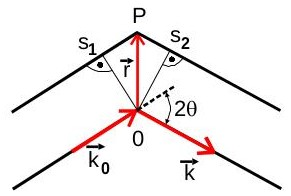
\includegraphics[width=0.4\textwidth]{abb8.jpg}
\caption{Geometrische Überlegung zur Berechnung des Phasenunterschiedes $\Delta \varphi$ zweier Wellen die an den Punkten O und P gestreut werden. Abbildung entnommen aus \cite{V41}.}
\label{abb:8}
\end{wrapfigure}
Durch geometrische Überlegungen, welche in Abbildung \ref{abb:8} dargestellt sind, wird deutlich, dass der Phasenunterschied
\begin{equation}
  \label{eq:7}
  \Delta \varphi=2\pi \frac{\Delta s}{\lambda}=2\pi \frac{s_1+s_2}{\lambda}=2\pi\vec r \cdot \left(\vec k- \vec k_0\right)
\end{equation}
beträgt.
Um nun die Streuung am Kristallgitter zu beschreiben, muss  der Phasenunterschied zwischen zwei Wellen, die an unterschiednlichen Atomen in der Elementarzelle gestreut werden, bekannt sein.
Wenn das eine Atom sich im Ursprung des Koordinatensystems befindet und sich der Platz des anderen Atoms durch den Ortsvektor $\vec r_j$ beschreiben lässt, beträgt diese Phasendifferenz
\begin{equation}
  \Delta \varphi_j = 2\pi \vec r_j\cdot \left(\vec k-\vec k_0\right).
\end{equation}
Die gesamte Streuamplitude $A$ berechnet sich durch die Summe aller einzelnen Intensitäten:
\begin{equation}
  A=\sum_jf_j\exp\left(-2\pi i \vec r _j\cdot\left(\vec k-\vec k_0\right)\right)I_\text{e},
\end{equation}
wobei $f_j$ der Formfaktor des entsprechendes Atoms ist.
Stellt man nun die Ortsvektoren durch die Basisvektoren $\vec a_i$ dar, erhält man die Strukturamplitude
\begin{equation}
  S=\sum_jf_j\exp\left(-2\pi i \left(x_j\vec a_1+x_j\vec a_2+x_j\vec a_3 \right)\cdot\left(\vec k-\vec k_0\right)\right)I_\text{e}.
\end{equation}
Dabei gilt für die Beträge der Basisvektoren $|\vec a_i|\le 1$.
Das Betragsquadrat der Strukturamplitude  $|S^2|=SS^*$ heißt Strukturfaktor und gibt das Verhältnis von einer Elementarzelle und von einem einzelnen Elektron gestreuten Intensitäten an.
Um Streuung an Elementarzellen, die in einem periodischen Gitter angeordnet sind, zu betrachten, wird eine Elementarzelle als punktförmig angenommen, sodass die Bragg-Bedingung
\begin{equation}
  n\lambda=2d\sin\left(\theta\right)~~~\text{mit}~n=1,2,...
\end{equation}
gilt.
Diese Bragg-Bedingung kann auch durch die Wellenzahlvektoren und den reziproke Gittervektor $\vec G$ dargestellt werden:
\begin{equation}
  \vec k -\vec k_0 =\vec G.
\end{equation}
Der reziproke Gittervektor
\begin{equation}
  \vec G= h g_1+kg_2+lg_3
\end{equation}
besteht aus den Millerschen Inzides $hkl$ und den Basisvektoren
\begin{equation}
   \vec g_1=\frac{\vec a_2\times \vec a_3}{\vec a_1 \cdot \left(\vec a_2 \times \vec a_3\right)}, ~~  \vec g_2=\frac{\vec a_3\times \vec a_1}{\vec a_1 \cdot \left(\vec a_2 \times \vec a_3\right)}~~\text{und}~~  \vec g_3=\frac{\vec a_1\times \vec a_2}{\vec a_1 \cdot \left(\vec a_2 \times \vec a_3\right)}
\end{equation}
des reziproken Gitters.
Die Strukturamplitude
\begin{equation}
  S(h,k,l)=\sum _j f_j\exp\left(x_j h+ y_jk+z_j l\right)
\end{equation}
berechnet sich nun in Abhängigkeit von den Millerschen Indizes und der Orte der Atome $\vec r_j=\left(x_j, y_j, z_j\right)^\text{T}$  in der Elementarzelle.
